\subsection{Logistic regression}
During the process of optimizing our logistic regression model for our NLP (Natural language processing) problem, we encountered multiple problems related to the nature of the task. The main issue was that the model didn’t consider the number of entries for each category of emotion. For example, there were a considerable number of "joy" entries, but only a few "surprise" entries. Consequently, the model had a tendency to choose "joy" over "surprise," even when we tried to influence it by entering words with high TF-IDF scores in the "surprise" category.
We optimized the model by adding weights to each category to balance the distribution across the six categories. This was achieved by introducing sklearn’s compute\_class\_weight method. This method considers all entries across the entire dataset and ensures that all emotions are represented equally. This, in turn, resolved the distribution issue in the predictions.
Another problem that arose was the model’s focus on individual words within a sentence rather than their coherence. This became the main focus of our optimization efforts. After conducting research, we decided to use n-grams, specifically ngram\_range of (1, 2). This approach considers pairs of words and takes into account the implications of combining two words and the associated emotion. \autocite{logistic-regression}

\begin{figure}[H]
    \centering
    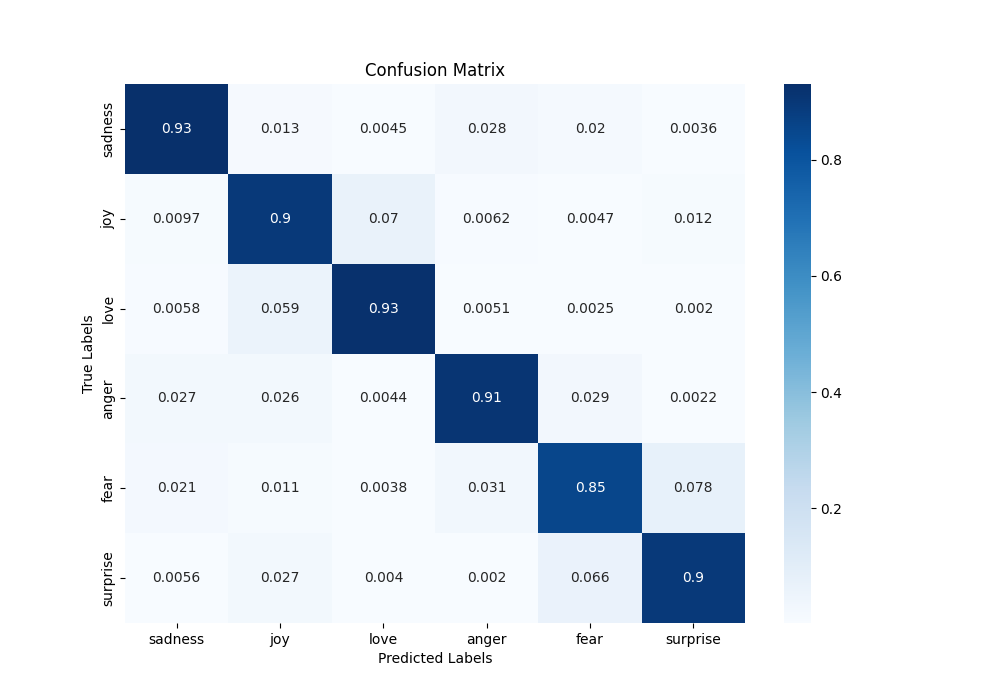
\includegraphics[width=1\columnwidth]{images/Confusion_matrix.png}
    \caption{Confusion matrix showing a 90\% average score in correlation between true and predicted labels. Most significant misclassifications exists between joy and love}
    \label{fig:correlation_plot}
\end{figure}

\begin{figure}[H]
    \centering
    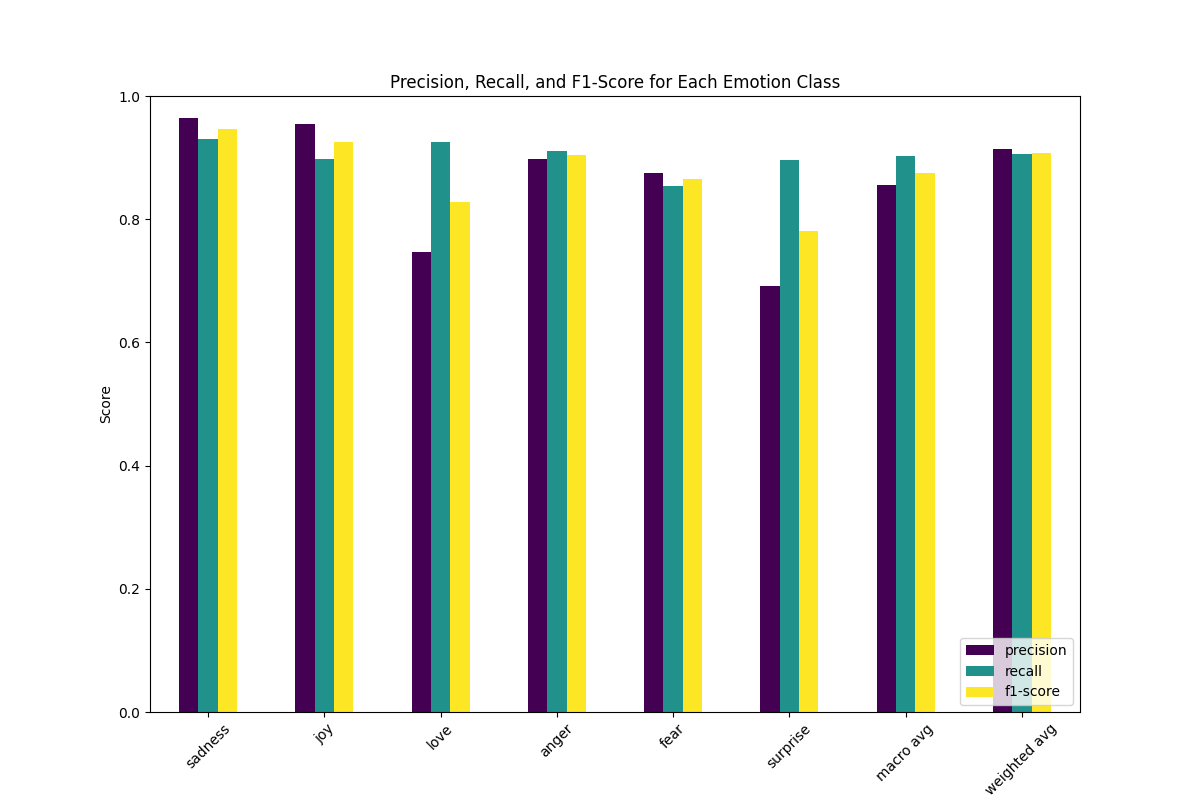
\includegraphics[width=1\columnwidth]{images/Classification_report_model1.png}
    \caption{Classification report based on our Logistic regression model. Emotions across the board showing mostly above 0.8, which indicates strong model performance across these metrics}
    \label{fig:correlation_plot}    
\end{figure}

